%% ======================================================================
%% AAAI-27 WORKSHOP PAPER
%% ----------------------------------------------------------------------
%% HOW TO USE ON OVERLEAF
%%  1. Download the official AAAI-27 Author Kit: https://aaai.org/authorkit27/
%%  2. Upload the kit's .sty and .bst files (e.g., aaai2027.sty, aaai2027.bst)
%%     to your Overleaf project root, next to this main.tex.
%%  3. Set Overleaf compiler to pdfLaTeX (Menu -> Compiler).
%%  4. Put figures in a folder called figures/ and references in aaai2027.bib.
%%
%% AAAI STYLE RULES (violations can get a paper rejected):
%%  - Do NOT load: geometry, fullpage, hyperref, titlesec, savetrees,
%%    authblk, layout, CJK, etc.
%%  - Do NOT change margins, font sizes, \baselinestretch, column spacing,
%%    or use negative \vspace to squeeze text.
%%  - US Letter paper, two columns, Type 1 / TrueType fonts only.
%%  - AAAI requires the submission source to be a SINGLE .tex file.
%% ======================================================================

\def\year{2027}\relax
\documentclass[letterpaper]{article} % DO NOT CHANGE THIS

%% --- Choose ONE of the two lines below --------------------------------
\usepackage[submission]{aaai2027}  % anonymous review version
% \usepackage{aaai2027}            % camera-ready version
%% ----------------------------------------------------------------------

\usepackage{times}        % DO NOT CHANGE THIS
\usepackage{helvet}       % DO NOT CHANGE THIS
\usepackage{courier}      % DO NOT CHANGE THIS
\usepackage[hyphens]{url} % DO NOT CHANGE THIS
\usepackage{graphicx}     % DO NOT CHANGE THIS
\urlstyle{rm}             % DO NOT CHANGE THIS
\def\UrlFont{\rm}         % DO NOT CHANGE THIS
\usepackage{natbib}       % DO NOT CHANGE THIS
\usepackage{caption}      % DO NOT CHANGE THIS
\frenchspacing            % DO NOT CHANGE THIS
\setlength{\pdfpagewidth}{8.5in}  % DO NOT CHANGE THIS
\setlength{\pdfpageheight}{11in}  % DO NOT CHANGE THIS

%% --- Safe, commonly used extra packages -------------------------------
\usepackage{algorithm}
\usepackage{algorithmic}
\usepackage{amsmath}
\usepackage{amssymb}
\usepackage{booktabs}     % nicer tables (\toprule, \midrule, \bottomrule)
\usepackage{multirow}
\usepackage{xcolor}
\usepackage{tikz}
\usetikzlibrary{arrows.meta,positioning}
\usepackage{pifont}
\usepackage{newfloat}
\usepackage{listings}
\DeclareCaptionStyle{ruled}{labelfont=normalfont,labelsep=colon,strut=off}
\lstset{%
  basicstyle={\footnotesize\ttfamily},
  numbers=left,numberstyle=\footnotesize,xleftmargin=2em,
  aboveskip=0pt,belowskip=0pt,
  showstringspaces=false,tabsize=2,breaklines=true}
\floatstyle{ruled}
\newfloat{listing}{tb}{lst}{}
\floatname{listing}{Listing}

%% --- Handy macros -----------------------------------------------------
\newcommand{\method}{\textsc{ESV}}   % your method's name
%% \cost shades the small "what this costs" line inside the figure boxes.
%% (The tikz key cost/.style is a node style, not this macro: both are used.)
\newcommand{\cost}{\scriptsize}

%% --- Plot helpers for the result figures (native TikZ, no bitmaps) ----
%% Marker shapes are core TikZ nodes, so every glyph is vector and uses the
%% document's Type 1 text fonts: no Type 3 subsets, no raster, nothing to crop.
\definecolor{pblue}{RGB}{31,97,160}
\definecolor{pgreen}{RGB}{0,122,87}
\definecolor{pgrey}{RGB}{95,95,95}
\newcommand{\mkopensq}[2]{\node[draw=#2,fill=white,line width=.6pt,rectangle,inner sep=1.5pt] at #1 {};}
\newcommand{\mkfillsq}[2]{\node[draw=#2,fill=#2,rectangle,inner sep=1.5pt] at #1 {};}
\newcommand{\mkopenci}[2]{\node[draw=#2,fill=white,line width=.6pt,circle,inner sep=1.5pt] at #1 {};}
\newcommand{\mkfillci}[2]{\node[draw=#2,fill=#2,circle,inner sep=1.5pt] at #1 {};}
%% #1 x, #2 centre, #3 half-width of the interval, #4 color (needs x=1cm)
\newcommand{\ebar}[4]{%
  \draw[#4,line width=.5pt] (#1,{#2-#3}) -- (#1,{#2+#3});
  \draw[#4,line width=.5pt] ({#1-0.055},{#2-#3}) -- ({#1+0.055},{#2-#3});
  \draw[#4,line width=.5pt] ({#1-0.055},{#2+#3}) -- ({#1+0.055},{#2+#3});}

%% --- Comparison-table glyphs ------------------------------------------
\definecolor{okgreen}{RGB}{0,122,87}
\definecolor{okred}{RGB}{176,42,32}
\newcommand{\yes}{\textcolor{okgreen}{\ding{51}}}
\newcommand{\no}{\textcolor{okred}{\ding{55}}}
\newcommand{\na}{\textcolor{black!45}{--}}

%% --- Figure fills (shaded by cost) ------------------------------------
\definecolor{cshared}{RGB}{226,226,226}
\definecolor{ccode}{RGB}{205,228,243}
\definecolor{ccall}{RGB}{252,230,192}
\definecolor{ccallb}{RGB}{191,118,0}
\definecolor{cout}{RGB}{206,238,227}
\definecolor{ctrap}{RGB}{250,222,218}

%% PDF metadata: leave Title/Author EMPTY for anonymous submission
\pdfinfo{
/TemplateVersion (2027.1)
}

\setcounter{secnumdepth}{1} % 0 = unnumbered sections (AAAI default)

%% --- Float placement --------------------------------------------------
%% Default LaTeX stretches a float-only page with infinite glue, which opens
%% large blank bands between stacked tables. Top-align and pack them instead.
%% Nothing here changes margins, type size, leading or column separation.
\makeatletter
\setlength{\@fptop}{0pt}
\setlength{\@fpsep}{12pt plus 0fil}
\setlength{\@fpbot}{0pt plus 1fil}
\setlength{\@dblfptop}{0pt}
\setlength{\@dblfpsep}{12pt plus 0fil}
\setlength{\@dblfpbot}{0pt plus 1fil}
\makeatother
%% A page of pure floats must be nearly full to be worth making, so tables
%% prefer to share a page with text.
\renewcommand{\floatpagefraction}{0.85}
\renewcommand{\dblfloatpagefraction}{0.85}

%% ======================================================================
%% TITLE & AUTHORS
%% ======================================================================
\title{Explicit Strategy Verification:\\ Verify the Strategy, Not the Vote --- Gold-Free Answer Selection Without Re-Solving}

%% In submission mode the style hides authors automatically, but keep
%% this block filled in so camera-ready is one switch away.
%%\author{
%%    Ekansh Agrawal\textsuperscript{\rm 1},
%%    Ritvij Sharma\textsuperscript{\rm 1},
%%    Anand Jayshree Ramaswamy\textsuperscript{\rm 1}
%%}
%%\affiliations{
%%    ekansh2023@tamu.edu, ritvij.starspark.ai, anand@arizona.edu
%%}

%% Uncomment if your workshop is NOT published in AAAI proceedings
%% (most workshops) -- removes the AAAI copyright notice.
% \nocopyright

\begin{document}
\affiliations{Institution Name, City, Country}

\maketitle

%% ======================================================================
%% ABSTRACT  (aim for ~150--250 words, one paragraph, no citations)
%% ======================================================================
\begin{abstract}
Self-consistency samples several chains of thought and returns the majority
answer. It is the standard way to turn extra inference compute into accuracy on
reasoning and logic benchmarks, but it selects by answer frequency alone, so it
cannot see whether the reasoning behind any candidate is valid, and its accuracy
falls sharply as the problems get harder. For small open-weight models, the best
answer already present among the four sampled chains of thought
beats their majority vote by 6 points on GSM8K, 12 on MATH-500 and 18 on
JEEBench. We introduce \textbf{\method{}}, \textbf{E}xplicit \textbf{S}trategy \textbf{V}erification, a gold-free procedure that never re-solves the problem: a zero-cost disagreement gate, one contrastive
verification call that requires each candidate's strategy to be bound to quoted givens and its preconditions checked, and a deterministic rule that accepts only
candidates with no mismatched binding and no violated condition. Across 2,918 instances spanning GSM8K, MATH-500 and JEEBench, \method{} improves accuracy by 5.0, 5.9 and 3.5 points over CoT maj@4 (148 repairs against 4 regressions; $p \le 10^{-7}$ on all three), while Universal Self-Consistency reaches significance
on none. Substituting the solver for the stronger checker reverses the
effect on all three benchmarks, which pins down what the method needs: gold-free
verification requires a verifier stronger than the model under test. Every problem is paired with a
structural perturbation that either breaks the strategy the original invites or
preserves it. This design manufactures selection errors of known cause and
separates strategy misfit from mere novelty, the error class frequency-based
selection cannot see.
\end{abstract}

%% ================================================
\section{Introduction}

Large language models solve multi-step reasoning problems by generating an
explicit chain of thought before committing to an answer~\cite{wei2022chain}. Because any single chain can go wrong, the standard
way to spend additional inference compute is to sample several of them and return their majority answer, a procedure known as self-consistency~\cite{wang2022self}. But majority voting selects among candidates by answer frequency alone, so it cannot see whether the reasoning that produced any of them is valid. What that forfeits is
substantial: for small open-weight models, the best answer already present among four sampled chains of thought exceeds their majority vote by six points on GSM8K, twelve points on MATH-500 and eighteen points on JEEBench. Existing gold-free remedies take one of two routes. One re-solves the problem from a critique of the first attempt~\cite{madaan2023self,shinn2023reflexion}; the other asks the model to nominate the most consistent of its own samples~\cite{chen2023universal}. The first pays full inference cost a second
time, and the second inherits the biases that produced the error.

A practical gold-free selection method has to satisfy three
requirements at once: (1) it must never consult a reference answer, so
that it is deployable at inference time; (2) it must not re-solve the problem,
so that its cost is a fraction of the sampling budget it augments rather than a
multiple of it; and (3) it must not damage answers that were already correct,
since a method that fires on uncertainty can break a correct majority as easily
as repair a wrong one (Section~\ref{sec:requirements}). Existing methods satisfy
at most two. Re-solving approaches violate (2) by construction, and when the
model critiques its own work they violate (3) as well, because the blind spot
that produced the error also confirms it~\cite{huang2024large}. Selection
methods such as Universal Self-Consistency respect (1) and (2), but they ask the
solver to adjudicate its own samples, and so gain little over the majority vote
they replace.

We propose \textbf{\method{}} (\textbf{Explicit Strategy
Verification}), a multi-stage gold-free pipeline that selects among answers the
solver has already produced and never re-solves the problem
(Section~\ref{sec:method}). A disagreement
gate first groups the samples into distinct candidates and halts as soon as
they agree, which costs no model calls and puts all verification
spend on the instances that can actually change. Where they disagree, a single call hands the
distinct candidates, deduplicated and with their vote counts hidden, to a checker
stronger than the solver, and a decision rule either commits to one candidate or
abstains and keeps the majority answer. On
GSM8K, MATH-500 and JEEBench, across three open-weight solvers on the first and
two on the others, \method{} improves accuracy over majority voting by 5.0, 5.9
and 3.5 points respectively, against 0.9, 0.4 and $-1.9$ points for Universal
Self-Consistency, at 44\%, 83\% and 100\% of the sampling budget in additional
compute. To attribute the gain, we evaluate each stage in isolation on a
benchmark of structural perturbations we built for the purpose.

Our contributions are:
\begin{itemize}
  \item We set out three requirements that a gold-free selection method must
        meet jointly, and show that no existing method meets all three.
  \item We propose \method{}, a gated verification pipeline that improves on
        majority voting and Universal Self-Consistency on every benchmark and
        solver we evaluate, without re-solving any problem.
  \item We construct a perturbation benchmark of matched problem pairs in which
        one variant breaks the strategy the original invites and the other
        preserves it, with an independently verified trap answer that makes the
        cause of each failure known.
  \item Component-wise experiments trace the gain to the checker's strength
        rather than to the verification format, and show that substituting the
        solver for the checker reverses the method's effect entirely.
\end{itemize}

%% ======================================================================
\section{Related Works}
%% ======================================================================
% Group by theme, not paper-by-paper. End each group with how you differ.
We group related work under five themes: sampling and answer
aggregation, self-correction, external verification and LLM judges,
perturbation robustness, and test-time compute allocation.

\paragraph{Sampling and answer aggregation.}
Self-consistency samples several chains of thought and returns the modal answer
\cite{wang2022self}, and later work generalises the vote to free-form
outputs by asking the model itself to select the most consistent response
\cite{chen2023universal}. Agreement governs aggregation of this kind
completely: the answer a plurality of samples reach is returned whether or not
its derivation is sound, so errors shared across samples are
unrecoverable and a correct answer appearing only once can never win. We instead
leave the sample budget untouched and replace the frequency
statistic with an explicit soundness check over the distinct candidates, which
lets a minority answer win when the majority's reasoning does not
survive verification.

\paragraph{Self-correction and its limits.}
Prior work on iterative refinement has models critique and revise their own
outputs \cite{madaan2023self, shinn2023reflexion}, while a growing body of
negative results finds that, with no external signal, language models cannot
reliably identify errors in their own reasoning \cite{huang2024large}. These
studies establish \emph{that} self-correction fails; they do not isolate the
quantity responsible. We measure it directly. Holding the candidate set, the
prompt and the decision rule fixed and varying only the identity of the checker,
we find that a solver judges its own derivations sound an order of magnitude
more often than an independent checker does, and that this miscalibration, rather
than the verification format, is what turns self-checking into a net loss.

\paragraph{Learned verifiers and LLM judges.}
A complementary line trains or prompts a separate model to assess candidate
solutions, as an outcome verifier \cite{cobbe2021training}, a step-level process
reward model \cite{lightman2024let}, or a general-purpose judge
\cite{zheng2023judging}. This work establishes that external scoring helps, but
it conflates two factors: how capable the checker is, and the form in which it
is asked to deliberate. We separate them with a control that holds the checker,
its candidates and its budget fixed while replacing structured verification with
free-form adjudication, and we report that comparison in both directions,
including the regimes where the structured form is the weaker of the two.

\paragraph{Perturbation and the memorization question.}
Robustness studies perturb benchmark problems to test whether apparent reasoning
survives distribution shift, by resampling symbolic templates, altering numeric
values, or inserting insignificant clauses \cite{mirzadeh2025gsm}. Such
perturbations stay largely at the surface and carry no annotation with respect to
the solution procedure, so a drop in accuracy cannot be traced to any
specific failure of transfer. We define perturbations relative to an explicit
solution strategy extracted from the original problem, and label each pair
strategy-breaking or strategy-preserving only after two independent verifiers
agree on the perturbed answer and confirm what that particular strategy does to it.
For breaking pairs we also record the trap answer the original strategy
yields, which gives per-instance ground truth for the error mode a selector has to
detect.

\paragraph{Allocating test-time compute.}
Recent work treats inference-time computation as a resource to be scheduled,
trading additional samples, search, or verifier calls against accuracy \cite{snell2024scaling}. Our method is deliberately frugal within this framing: verification is gated on disagreement among the existing samples, so no
additional call is issued where the solver is already unanimous, and the checker
is invoked at most once per instance. We report the resulting cost in full,
giving billed and critical-path latency, solver and verifier tokens separately, and
tokens per net correction, so that the accuracy gained can be weighed against
simply drawing more samples.

%% ======================================================================
\section{Preliminaries and Problem Formulation}
\label{sec:prelim}
%% ======================================================================

\paragraph{Sampling and candidates.}
Given a problem $x$ with reference answer $y$, a solver produces $n = 4$ chains
of thought and the answer each one reaches. Grouping answers that agree under a
type-aware normalization yields $K \le n$ distinct \emph{candidates}
$c_1, \dots, c_K$ with vote counts $v_1, \dots, v_K$ summing to $n$, each
carrying one representative solution. Self-consistency \cite{wang2022self}
returns the candidate with the most votes, which we write $m(x)$ and refer to
throughout as CoT maj@4, our baseline. We write CoT pass@4 for the oracle that
is correct whenever $y$ appears among the candidates.

\paragraph{The selection task.}
We study \emph{answer selection}: given the problem and the candidates the
solver has already produced, commit to one of them. Every method we compare
consumes the same four samples, drawn once per instance and reused unchanged,
and differs only in the evidence it reads off them. CoT maj@4 uses the vote
counts; Universal Self-Consistency \cite{chen2023universal} sees the samples
with duplicates shown, so multiplicity remains visible; the verification
methods we study see the problem text and the representative solutions with
vote counts withheld. Holding the input fixed in this way makes the comparison
one about selection evidence rather than about sampling luck.

\subsection{Requirements on a gold-free selector}
\label{sec:requirements}

Three constraints separate a selector deployable at inference time from one
that merely explains a benchmark after the fact.

\begin{description}
\item[\textnormal{(R1) \emph{Gold-free.}}] The selector reads only the problem
  and the samples. The reference answer enters at scoring and nowhere else.
\item[\textnormal{(R2) \emph{No re-solving.}}] The selector issues no further
  call to the solver, so its cost is a fraction of the sampling budget it
  augments rather than a multiple of it.
\item[\textnormal{(R3) \emph{Non-destructive.}}] Because the selector may
  overturn $m(x)$, it must be judged by what it repairs \emph{and} what it
  damages, not by accuracy alone.
\end{description}

R3 fixes our unit of measurement. Against the maj@4 baseline, a \emph{fix} is
an instance the majority got wrong and the selector gets right, a \emph{break}
the reverse, and we report the two together with an exact McNemar test rather
than an accuracy delta on its own.

\paragraph{Selection is a two-sided bet.}
A selector constrained to the candidates cannot invent an answer the solver
never produced, which bounds both of its tails. Let $\mathcal{F}$ be the
instances where the majority is wrong but some candidate is right, and
$\mathcal{B}$ those where the majority is already right and the candidates
disagree. Over $N$ instances,
\begin{equation}
  -\frac{|\mathcal{B}|}{N}
  \;\le\; \Delta\mathrm{acc}
  \;\le\; \frac{|\mathcal{F}|}{N}
  \;=\; \mathrm{pass@}4 - \mathrm{maj@}4 ,
  \label{eq:bounds}
\end{equation}
since a unanimous-but-wrong instance contains no correct candidate and so
raises neither bound. The upper bound is the \emph{headroom} a selector
competes for. The two sets are not the same size, and we report both in
Section~\ref{sec:results}; the relevant point here is that R3 is forced by
Eq.~\eqref{eq:bounds} rather than adopted out of caution.

\paragraph{When a verdict is worth acting on.}
The vote is itself an informative signal, so a selector that overturns it needs
evidence strong enough to overcome that prior. Let $p(v)$ be the probability
that a candidate with $v$ votes is correct and
$\rho(v) = p(v)/(1 - p(v))$ the corresponding odds. A verifier returning
evidence $E$ about a candidate carries the likelihood ratio
$\Lambda = \Pr(E \mid \text{correct}) / \Pr(E \mid \text{wrong})$, and
preferring a $v_c$-vote candidate over a $v_m$-vote majority requires
\begin{equation}
  \Lambda \;>\; \rho(v_m) \,/\, \rho(v_c) .
  \label{eq:threshold}
\end{equation}
We estimate $p(v)$ on a development split of one benchmark and hold the
resulting thresholds fixed thereafter, so Eq.~\eqref{eq:threshold} states in
advance how strong a checker must be before a verification call can pay for
itself. It is a specification fixed before any verifier is measured, not a
post-hoc account of one, and Section~\ref{sec:results} compares measured
likelihood ratios against it.

\paragraph{Perturbation pairs.}
Rather than evaluate on problems whose failure modes are unknown, we evaluate
on matched pairs. Each item is a frozen pair $(P, P')$ together with the
solution strategy $S$ that the original invites, where $P'$ alters one
structure, relationship or constraint of $P$ while remaining well posed and
keeping the original answer format. In a \emph{strategy-breaking} pair,
applying $S$ unchanged to $P'$ gives a wrong answer, which we record as the
\emph{trap}; in a \emph{strategy-preserving} pair, $S$ still works but the
answer changes and must be recomputed. The preserving mode is the control for
mere novelty, separating a method that degrades on any altered problem from one
that detects strategy misfit. The trap is what makes a pair informative: a
candidate equal to the trap is wrong for a known reason, which supplies
per-instance ground truth for the error class that frequency-based selection
cannot see. Section~\ref{sec:setup} gives the generation and verification
protocol and the resulting dataset statistics.

%% ======================================================================
\section{Method}
\label{sec:method}
%% ======================================================================

We describe the method in the order it runs: first how a perturbation pair is
built and frozen, then the stages that turn four samples into one committed
answer, then the selectors we compare against.
Figure~\ref{fig:overview} places all five methods on the one sampling step they
share, Figure~\ref{fig:pipeline} opens up \method{} itself, and
Table~\ref{tab:methods} states what each selector is allowed to see and do.

\begin{figure*}[t]
\centering
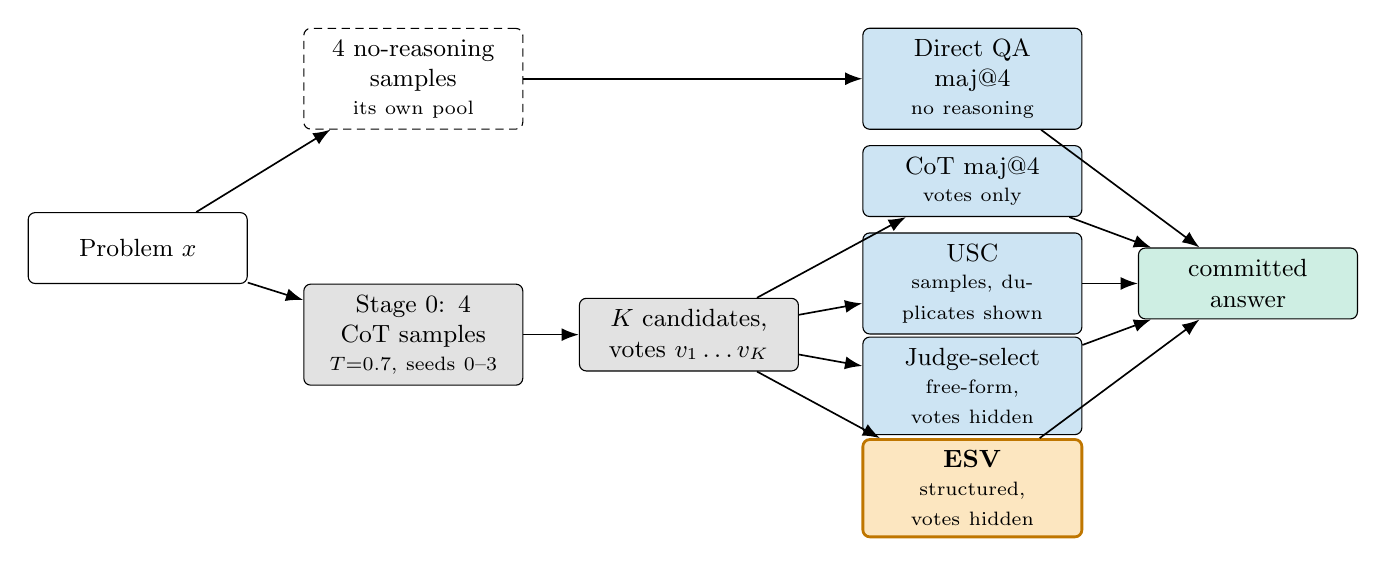
\begin{tikzpicture}[
  font=\small,
  %% text width is fixed, so no box can grow into a neighbour's gap
  base/.style={draw, rounded corners=2.5pt, align=center, inner sep=4pt,
               text width=25mm, minimum height=9mm},
  input/.style={base, fill=white},
  shared/.style={base, fill=cshared},
  own/.style={base, fill=white, densely dashed},
  sel/.style={base, fill=ccode},
  ours/.style={base, fill=ccall, draw=ccallb, line width=1pt},
  outbox/.style={base, fill=cout},
  ar/.style={-{Latex[length=2.2mm]}, semithick},
  cost/.style={font=\scriptsize},
]
\node[input]  (prob)  at (0,-0.2)     {Problem $x$};
\node[own]    (dpool) at (3.5,1.95)   {$4$ no-reasoning samples\\[-1pt]{\cost its own pool}};
\node[shared] (pool)  at (3.5,-1.3)   {Stage~0: $4$ CoT samples\\[-1pt]{\cost $T{=}0.7$, seeds $0$--$3$}};
\node[shared] (cands) at (7.0,-1.3)   {$K$ candidates, votes $v_1 \dots v_K$};

\node[sel]    (dqa)   at (10.6,1.95)  {Direct QA maj@4\\[-1pt]{\cost no reasoning}};
\node[sel]    (maj)   at (10.6,0.65)  {CoT maj@4\\[-1pt]{\cost votes only}};
\node[sel]    (usc)   at (10.6,-0.65) {USC\\[-1pt]{\cost samples, duplicates shown}};
\node[sel]    (jud)   at (10.6,-1.95) {Judge-select\\[-1pt]{\cost free-form, votes hidden}};
\node[ours]   (esv)   at (10.6,-3.25) {\textbf{\method{}}\\[-1pt]{\cost structured, votes hidden}};

\node[outbox] (ans)   at (14.1,-0.65) {committed answer};

\draw[ar] (prob)  -- (dpool);
\draw[ar] (prob)  -- (pool);
\draw[ar] (dpool) -- (dqa);
\draw[ar] (pool)  -- (cands);
\draw[ar] (cands) -- (maj);
\draw[ar] (cands) -- (usc);
\draw[ar] (cands) -- (jud);
\draw[ar] (cands) -- (esv);
\draw[ar] (dqa)   -- (ans);
\draw[ar] (maj)   -- (ans);
\draw[ar] (usc)   -- (ans);
\draw[ar] (jud)   -- (ans);
\draw[ar] (esv)   -- (ans);
\end{tikzpicture}
\caption{How the methods relate. One stage~0 pool (grey) is drawn per instance
and read unchanged by four of the five selectors, so the comparison is about
selection evidence rather than sampling luck. Direct QA is the exception: it
draws its own samples from a prompt that forbids reasoning (dashed), and is a
floor on recall rather than a selector. The four selectors differ only in what
they read off the pool. Every path commits to a candidate the solver already
produced, so CoT pass@4 is a hard ceiling throughout.}
\label{fig:overview}
\end{figure*}

\subsection{Constructing the perturbation pairs}
\label{sec:construction}

One generator model produces each pair, and two verifier models have to agree
before it is accepted. The verifiers are independent of the generator and of
each other, and none of the three is a solver in any later experiment. One of
the two verifiers is, however, the same model we later use as the independent
checker, so every perturbed problem in the dataset is one that checker answered
correctly during construction. That is why we report the originals separately:
they carry no such acceptance filter, and the checker's gain over the
vote has to survive on them as well (Section~\ref{sec:results}).

\paragraph{Generation.}
Given an original problem $P$ and its reference answer, the generator names the
solution strategy $S$ that $P$ invites, alters exactly one condition, and
returns the perturbed problem $P'$ together with its new answer, the condition
it changed, the reason the change matters, an alternative strategy, the answer
$S$ would produce if applied unchanged, and a confidence level. A balancer
assigns each problem one mode, strategy-breaking or strategy-preserving,
before the first attempt and holds it across retries. This keeps the two modes
near parity instead of letting the generator drift toward whichever is easier
to produce.

\paragraph{Verification.}
Acceptance turns on two calls to each verifier, in an order chosen so that
anchoring is impossible.

\begin{description}
\item[\textnormal{\emph{Blind solve.}}] The verifier sees $P'$ alone, without
  $P$, without $S$ and without the generator's answer, and solves it. The pair is
  rejected if the verifier declares $P'$ ill-posed, if its answer disagrees
  with the generator's, or if its confidence falls below $0.6$. Withholding $P$
  is what makes the resulting answer an independent check rather than a
  ratification.
\item[\textnormal{\emph{Mechanical strategy application.}}] The verifier now
  sees $P$, $P'$, $S$ and the verified answer, and applies $S$ to $P'$ without
  adapting it. In breaking mode the pair is confirmed when the resulting answer
  differs from the verified answer; in preserving mode, when it agrees. A
  report that $S$ cannot be carried out at all counts as a soft confirmation of
  breaking.
\end{description}

A pair is frozen only if neither verifier objects and at least one returns a
concrete confirmation; a soft confirmation alone is never sufficient. Rejected
attempts are returned to the generator with the objection attached and retried
up to a cap, and every attempt is logged so that the frozen set can be rebuilt
from the log.

\begin{figure}[t]
\centering
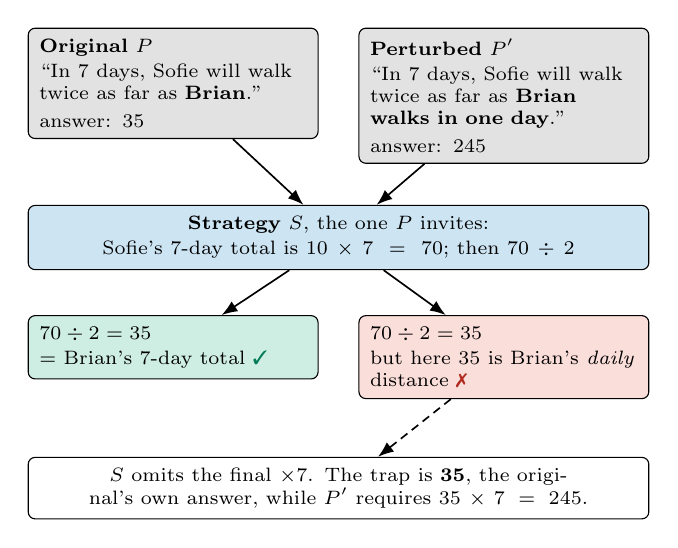
\begin{tikzpicture}[
  font=\scriptsize,
  base/.style={draw, rounded corners=2.5pt, align=left, inner sep=4pt,
               text width=34mm, anchor=north},
  wide/.style={base, text width=76mm, align=center},
  prob/.style={base, fill=cshared},
  strat/.style={wide, fill=ccode},
  good/.style={base, fill=cout},
  bad/.style={base, fill=ctrap},
  note/.style={wide, fill=white},
  ar/.style={-{Latex[length=2mm]}, semithick},
]
\node[prob] (pl) at (-2.1,0)
  {\textbf{Original $P$}\\[1pt]
   ``In 7 days, Sofie will walk twice as far as \textbf{Brian}.''\\[2pt]
   answer: $35$};
\node[prob] (pr) at (2.1,0)
  {\textbf{Perturbed $P'$}\\[1pt]
   ``In 7 days, Sofie will walk twice as far as \textbf{Brian walks in one
   day}.''\\[2pt]
   answer: $245$};

\node[strat] (s) at (0,-2.25)
  {\textbf{Strategy $S$}, the one $P$ invites:\\[1pt]
   Sofie's 7-day total is $10 \times 7 = 70$; then $70 \div 2$};

\node[good] (tl) at (-2.1,-3.65)
  {$70 \div 2 = 35$\\[1pt]
   $=$ Brian's 7-day total~\yes};
\node[bad] (tr) at (2.1,-3.65)
  {$70 \div 2 = 35$\\[1pt]
   but here $35$ is Brian's \emph{daily} distance~\no};

\node[note] (cc) at (0,-5.45)
  {$S$ omits the final $\times 7$. The trap is $\mathbf{35}$, the original's
   own answer, while $P'$ requires $35 \times 7 = 245$.};

\draw[ar] (pl) -- (s);
\draw[ar] (pr) -- (s);
\draw[ar] (s) -- (tl);
\draw[ar] (s) -- (tr);
\draw[ar, densely dashed] (tr) -- (cc);
\end{tikzpicture}
\caption{A strategy-breaking pair (GSM8K \#131), abridged; both problems also
state that Brian's daily distance is constant. Applying $S$ unchanged to $P'$
runs to completion and returns $35$, so the perturbation turns the original's
correct answer into the trap. The generator and both verifier models
independently returned $245$ for $P'$ and $35$ as the naive answer, and both
verifiers marked $S$ invalid on $P'$. Repeated samples agree on $35$ precisely
because they share the strategy, which is what frequency-based selection cannot
see.}
\label{fig:trap}
\end{figure}

Figure~\ref{fig:trap} shows one accepted breaking pair. The perturbation moves
the comparison from Brian's seven-day total to his one-day distance, and the
original strategy still completes on $P'$ and still returns $35$, so $35$ is the
trap: any candidate equal to it is wrong for a reason recorded at construction
time.

\subsection{Explicit Strategy Verification}
\label{sec:esv}

\begin{figure}[t]
\centering
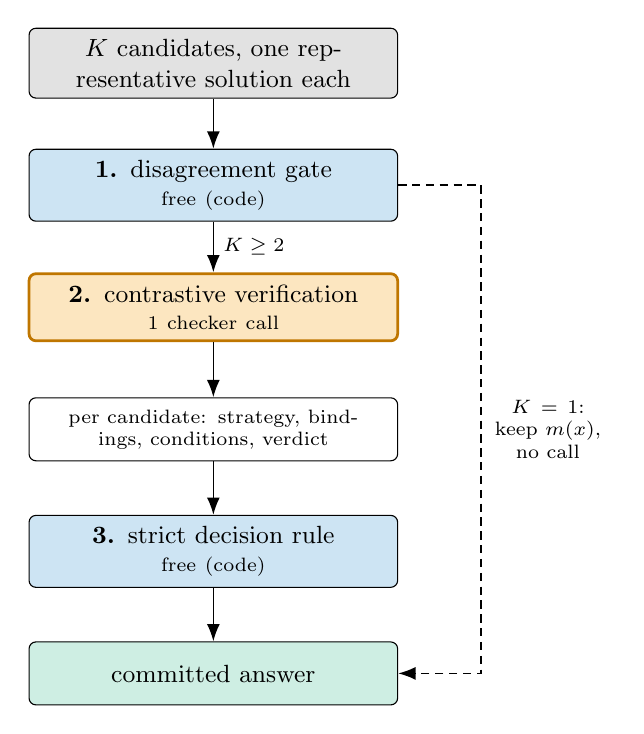
\begin{tikzpicture}[
  font=\small,
  base/.style={draw, rounded corners=2.5pt, align=center, inner sep=4pt,
               text width=44mm, minimum height=8mm},
  shared/.style={base, fill=cshared},
  code/.style={base, fill=ccode},
  call/.style={base, fill=ccall, draw=ccallb, line width=1pt},
  outbox/.style={base, fill=cout},
  fields/.style={base, fill=white, font=\scriptsize},
  ar/.style={-{Latex[length=2.2mm]}, semithick},
  cost/.style={font=\scriptsize},
  side/.style={font=\scriptsize, align=center, text width=15mm},
]
\node[shared] (cands) at (0,0)     {$K$ candidates, one representative solution each};
\node[code]   (gate)  at (0,-1.55) {\textbf{1.} disagreement gate\\[-1pt]{\cost free (code)}};
\node[call]   (ver)   at (0,-3.10) {\textbf{2.} contrastive verification\\[-1pt]{\cost $1$ checker call}};
\node[fields] (flds)  at (0,-4.65) {per candidate: strategy, bindings, conditions, verdict};
\node[code]   (rule)  at (0,-6.20) {\textbf{3.} strict decision rule\\[-1pt]{\cost free (code)}};
\node[outbox] (ans)   at (0,-7.75) {committed answer};

\draw[ar] (cands) -- (gate);
\draw[ar] (gate)  -- node[right, cost] {$K \ge 2$} (ver);
\draw[ar] (ver)   -- (flds);
\draw[ar] (flds)  -- (rule);
\draw[ar] (rule)  -- (ans);

%% unanimous bypass, routed down the right-hand margin
\coordinate (b1) at (3.4,-1.55);
\coordinate (b2) at (3.4,-7.75);
\draw[ar, densely dashed] (gate.east) -- (b1) -- (b2) -- (ans.east);
\node[side] at (4.25,-4.65) {$K = 1$:\\keep $m(x)$,\\no call};
\end{tikzpicture}
\caption{Inside \method{}, shaded by what each step costs. Two of the three
stages are deterministic code and free (blue); only contrastive verification
issues a model call (orange, heavy border), and only on the $K \ge 2$ instances
where the samples disagree. Unanimous instances take the dashed path and cost
nothing beyond sampling. The checker returns typed per-candidate fields rather
than a choice, and stage~3 reads those fields in code, so the model supplies
evidence and the rule supplies the decision.}
\label{fig:pipeline}
\end{figure}

\method{} adds three stages to a sampling step it shares with every other
method, and spends at most one model call on any instance.

\paragraph{Stage~0: shared sampling.}
Each solver answers each problem $n = 4$ times with chain-of-thought prompting
\cite{wei2022chain}, one call per sample at temperature $0.7$ under seeds $0$
to $3$, so that the four samples genuinely differ rather than repeating one
trajectory. Those four calls are the sampling budget against which every
later cost in this paper is measured. The samples are drawn once, written to
disk, and read unchanged by every selector, so no comparison below is affected
by sampling variance between methods.

\paragraph{Stage~1: the disagreement gate.}
The four answers are grouped into distinct candidates under a type-aware
normalization, in order of first appearance, with unreadable answers dropped.
If fewer than two candidates survive, the samples already agree, verification
has nothing to arbitrate, and the majority answer is committed with no call.
The gate is free and gold-free: it reads the samples only.

\paragraph{Stage~2: contrastive verification.}
Every surviving candidate is verified in a single call, each represented by one
of its solutions. The prompt states that the solutions reach different answers,
so at most one can be correct and all may be wrong; it presents them in
arbitrary order; and it withholds the vote counts while saying explicitly that
multiplicity is not evidence. For each candidate the checker returns the
strategy in one sentence, then one line per given the strategy depends on,
quoted word for word from the problem statement rather than from the solution's
restatement of it, marked \textsc{matches} or \textsc{mismatch}, then one
line per condition the strategy requires, marked \textsc{holds} or
\textsc{violated}. It then locates the first step at which the solutions
diverge, and finally returns \textsc{sound} or \textsc{flawed} per candidate
with a failure type, the first flawed step quoted verbatim, and the fact that
step should have asserted. Verification runs at temperature $0$. Asking for
quoted evidence before a verdict is the design choice under test. It is meant
to force the checker to commit to specific, checkable claims about the problem
text instead of judging fluency.

\paragraph{Stage~3: the decision rule.}
Selection is deterministic code with no further model call. Write $u_k$ for
candidate $k$'s verdict, $\mu_k$ for its count of \textsc{mismatch} bindings
and $\nu_k$ for its count of \textsc{violated} conditions. The candidate is
\emph{strictly sound} only if all three agree:
\begin{equation}
  \mathcal{S} = \{\, k : u_k = \textsc{sound},\; \mu_k = 0,\; \nu_k = 0 \,\}.
  \label{eq:strict}
\end{equation}
If $\mathcal{S}$ holds exactly one candidate, that candidate is committed. If it
holds several, the one with the most votes wins; ties go to the candidate
holding the majority answer $m(x)$, and then to the earliest in first-appearance
order. If it is empty, $m(x)$ is kept. The rule therefore never overturns the
baseline on evidence it does not have: where verification fails to discriminate,
\method{} returns what maj@4 would have returned, and the vote ranks only the
candidates verification has already cleared. Requiring the verdict to be
consistent with the checker's own line-by-line findings costs nothing and
discards verdicts the checker has already contradicted.

\paragraph{Two consequences of this shape.}
\method{} selects only among answers the solver already produced, so CoT pass@4
is a hard ceiling and no new answer can be introduced. And because an empty
$\mathcal{S}$ returns the majority answer, \method{} is a filter on
self-consistency rather than a replacement for it: it can only act where the
samples already disagree, and declines by default.

\paragraph{Checker conditions.}
We run stage~2 in two conditions that differ in nothing but which model is
called. Under \emph{self-check} the solver verifies its own samples; under
\emph{independent check} a single fixed checker verifies the samples of every
solver. Everything else (prompt, candidates, order, temperature, decision
rule) is held constant, so the contrast isolates the verifier.

\subsection{Methods compared}
\label{sec:comparisons}

\begin{table}[t]
\centering
\small
\setlength{\tabcolsep}{4pt}
\begin{tabular}{@{}lccccc@{}}
\toprule
 & DQA & maj@4 & USC & Judge & \textbf{\method{}} \\
\midrule
Gold-free             & \yes & \yes & \yes & \yes & \yes \\
Reads shared samples  & \no  & \yes & \yes & \yes & \yes \\
Votes hidden          & \na  & \na  & \no  & \yes & \yes \\
Can overturn $m(x)$   & \na  & \no  & \yes & \yes & \yes \\
May abstain           & \na  & \no  & \no  & \yes & \yes \\
Structured evidence   & \no  & \no  & \no  & \no  & \yes \\
\midrule
Extra calls           & $4^{\dagger}$ & $0$ & $1$ & $1$ & $1$ \\
\bottomrule
\end{tabular}
\caption{What each method may see and do. DQA is Direct QA, Judge the
judge-select control; \emph{structured evidence} means quoted bindings and
checked conditions rather than prose. A dash marks a property that presupposes
selecting among the shared candidates, which Direct QA and CoT maj@4 do not do.
The last two columns differ in one row only, so comparing them isolates
\method{}'s form from the checker's capability. $^{\dagger}$Direct QA draws its
own four samples from a no-reasoning prompt.}
\label{tab:methods}
\end{table}

Every selector consumes the stage~0 samples unchanged and differs only in the
evidence it reads off them. Table~\ref{tab:methods} sets out those differences.

\noindent\textbf{Direct QA} is the one arm that does not. It draws its own four
samples from a prompt that forbids reasoning and takes their majority, which
shows that the benchmarks are not solvable by recall.

\noindent\textbf{CoT pass@1} is the accuracy of a single sample, and
\textbf{CoT maj@4} \cite{wang2022self} the majority over four, which is our
baseline and the answer every selector must either confirm or overturn. \textbf{CoT
pass@4} marks an instance correct whenever any candidate is correct, giving the
oracle ceiling of Eq.~\eqref{eq:bounds}.

\noindent\textbf{Universal Self-Consistency} \cite{chen2023universal} is the
prior gold-free selector and our principal comparison. It receives all four
samples with duplicates shown, so consensus remains visible, and names the
sample it selects. Because an unresolved selection silently falls back to the
majority answer, we report the rate at which USC resolves a selection before
reporting its accuracy.

\noindent\textbf{Judge-select} is a form control, not a baseline. It is matched
to stage~2 on the checker, the candidates, their order, the withheld vote
counts, and the license to reject every candidate, and it reasons freely before
naming its pick. Two of those choices deliberately favor the control: free-form
reasoning makes the comparison structured-versus-unstructured rather than
reasoning-versus-none, and the license to decline denies \method{} a free win on
instances where no candidate survives. Judge-select therefore isolates what
\method{}'s structured form contributes once the checker's raw capability is
held fixed.

Reference answers enter at scoring and nowhere else, for every method.

%% ======================================================================
\section{Experimental Setup}
\label{sec:setup}

\paragraph{Datasets.}
We build pairs from GSM8K \cite{cobbe2021training}, MATH-500 \cite{hendrycks2021math,lightman2024let} and the mathematics questions of JEEBench \cite{arora2023jeebench}, sampling 200, 250 and 200 source problems with a fixed seed and running the protocol of Section~4. This freezes 198, 244 and 193 pairs, split almost evenly between breaking and preserving modes, with acceptance rates of 95--100\% per mode (Appendix~\ref{app:data}). MATH-500 keeps every answer format, including 88 symbolic expressions, which a normalizer compares identically for gold answers and for every method. Each pair contributes two instances, $P$ and $P'$, per solver. On GSM8K the decision rule and the checker were chosen on pairs 0--59 (357 instances) and evaluated once on pairs 60--197 (813 held-out instances), against a go/no-go criterion fixed beforehand: ESV must beat CoT maj@4 by at least 3 points and must beat USC. Six GSM8K originals with wrong or underdetermined published answers are excluded from every score. JEEBench served as the development benchmark for an earlier version of the pipeline, so we treat it as a third data point rather than held-out evidence.

\paragraph{Models.}
The solvers are Qwen2.5-7B-Instruct \cite{qwen2025qwen25}, Mistral-NeMo-12B and Gemma-3-4B-it \cite{gemma2025gemma3}, small enough that their majority vote leaves 6.1, 12.4 and 17.9 points of headroom below pass@4. Larger solvers leave 2.1 points on GSM8K and almost nothing to select (Appendix~\ref{app:large}). MATH-500 and JEEBench were run on Mistral-NeMo and Gemma-3-4B only. The independent checker is gpt-oss-120b \cite{openai2025gptoss}, a mixture-of-experts reasoning model with 116.8B total and 5.1B active parameters, shared by all solvers. Pairs were generated by DeepSeek-V4-Flash and accepted by Qwen3.5-35B-A3B and gpt-oss-120b. The checker's second role means every frozen $P'$ is one it solved correctly from $P'$ alone; originals escape this filter except through the few rejected pairs, and Section~\ref{sec:analysis} shows that the checker still gains on originals.

\paragraph{Baselines.}
CoT maj@4 \cite{wang2022self} is the answer every selector must overturn. Universal Self-Consistency \cite{chen2023universal} is the closest published gold-free selector: same four samples, one extra call, no re-solving. Direct QA tests whether the benchmarks yield to recall, and pass@4 is the ceiling of Eq.~(1). Self-check and judge-select are controls: the first removes the checker's advantage, the second removes ESV's structured form. Re-solving methods \cite{madaan2023self,shinn2023reflexion} violate R2 and are excluded.

\paragraph{Metrics.}
Against maj@4 on the same instances we count fixes $F$ and breaks $B$, report $\Delta = (F-B)/N$ with a 95\% paired interval, and test $F$ against $B$ with an exact two-sided McNemar test \cite{mcnemar1947}. Verifier quality is measured per candidate: TPR is the share of correct candidates judged strictly \textsc{sound}, FPR the share of wrong ones, and $\Lambda = \mathrm{TPR}/\mathrm{FPR}$ is compared against Eq.~(2). Cost is prompt plus completion tokens and critical-path latency (the four samples run concurrently; the extra call waits for them). The tests treat instances as independent, although instances from one source problem are correlated across solvers, so on GSM8K we also report each solver separately.

\paragraph{Implementation details.}
Nothing is trained; all models are queried through the OpenRouter API. Solvers draw four samples at temperature 0.7 with seeds 0--3 and a 4{,}000-token limit (6{,}000 on MATH-500). The checker, judge-select and USC run at temperature 0, with gpt-oss-120b at its default reasoning effort of medium. Malformed or truncated replies get one retry with a doubled limit, solutions shown to the checker are clipped to 6{,}000 characters, and numeric answers match within 0.01. We draw one set of samples per instance, so seed variance is not measured. Frozen data, all raw responses and the analysis code are released at the repository in Appendix~\ref{app:code}; every table regenerates offline from the stored responses.

%% ======================================================================
\section{Results}
\label{sec:results}
%% ======================================================================

\begin{table*}[t]
\centering
\small
\setlength{\tabcolsep}{4.2pt}
\begin{tabular}{lc rr rr rr}
\toprule
 & & \multicolumn{2}{c}{GSM8K (1{,}170; 3 solvers)} & \multicolumn{2}{c}{MATH-500 (976; 2 solvers)} & \multicolumn{2}{c}{JEEBench (772; 2 solvers)} \\
\cmidrule(lr){3-4}\cmidrule(lr){5-6}\cmidrule(lr){7-8}
Method & Calls & Acc.\ (\%) & $F$ / $B$ & Acc.\ (\%) & $F$ / $B$ & Acc.\ (\%) & $F$ / $B$ \\
\midrule
Direct QA maj@4 & 4$^\dagger$ & 12.1 & 7 / 900$^{***}$ & 10.7 & 22 / 468$^{***}$ & 11.9 & 57 / 150$^{***}$ \\
CoT pass@1 & 1 & 85.1 & & 51.6 & & 20.5 & \\
CoT maj@4 (baseline) & 4 & 88.5 & & 56.4 & & 24.0 & \\
Universal Self-Consistency & 4 + 1 & 89.3 & 19 / 9 & 56.8 & 34 / 30 & 22.0 & 32 / 47 \\
\midrule
ESV, self-check & 4 + 1 & 85.1 & 18 / 57$^{***}$ & 54.1 & 28 / 50$^{*}$ & 21.8 & 33 / 50 \\
ESV, gpt-oss-120b & 4 + 1 & 93.5 & 61 / 2$^{***}$ & 62.3 & 59 / 1$^{***}$ & 27.5 & 28 / 1$^{***}$ \\
Judge-select, gpt-oss-120b & 4 + 1 & \textbf{94.1} & 67 / 1$^{***}$ & \textbf{66.0} & 99 / 5$^{***}$ & \textbf{36.7} & 98 / 0$^{***}$ \\
\midrule
CoT pass@4 (oracle) & 4 & 94.5 & 71 / 0 & 68.8 & 121 / 0 & 41.8 & 138 / 0 \\
\bottomrule
\end{tabular}
\caption{Accuracy on the perturbation sets. $F$/$B$: fixes and breaks against CoT maj@4 on the same instances; exact McNemar $^{*}p<0.05$, $^{***}p<0.001$ (values in Appendix~\ref{app:pvalues}). ``4 + 1'': one extra call, issued only when the samples disagree. Judge-select is the form control (Section~4). Bold: best non-oracle method. $^\dagger$Direct QA draws its own four samples without reasoning.}
\label{tab:main}
\end{table*}

\subsection{Main Results}
\label{sec:main}

With gpt-oss-120b as checker, ESV improves on CoT maj@4 by 5.0, 5.9 and 3.5 points (Table~\ref{tab:main}; 61/2, 59/1 and 28/1 fixes against breaks, $p \le 10^{-7}$ each) and beats USC head to head by 53/4, 71/17 and 69/27. It passed the criterion fixed before the held-out run, reaching 94.1\% on the 813 held-out GSM8K instances against 88.8\% for maj@4 and 89.7\% for USC, and every GSM8K solver gains on its own (Qwen 91.0 to 94.6\%, NeMo 84.4 to 92.8\%, Gemma 90.0 to 93.1\%). USC does not significantly beat the majority vote on any benchmark ($p = 0.087$, $0.71$, $0.11$), and its 9 unresolved selections out of 303 on GSM8K (0 of 601 on MATH-500, 20 of 694 on JEEBench) are too few to explain that. Self-check ESV lowers accuracy on all three benchmarks ($-3.3$, $-2.3$ and $-2.2$ points; $p = 7\times10^{-6}$, $0.017$, $0.078$). Since self-check and the gpt-oss-120b configuration share the prompt, the candidates and the rule, the identity of the checker alone turns a loss into a gain, extending a known self-correction failure \cite{huang2024large} to a setting with no re-solving.

The form control shows where that gain comes from. Judge-select gives the same checker the same candidates without ESV's bindings, conditions or verdict form, and it is more accurate than ESV on every benchmark, by 0.6, 3.7 and 9.2 points (paired 7/0, 40/4 and 73/2; $p = 0.016$, $2\times10^{-8}$, $2\times10^{-19}$). Net of breaks it recovers 93, 78 and 71\% of the oracle headroom where ESV recovers 83, 48 and 20\% (Figure~\ref{fig:gain}). The accuracy comes from putting a stronger checker in front of the solver's own candidates; ESV's structured form contributes nothing to it and costs accuracy on harder problems.

\begin{figure}[t]
\centering
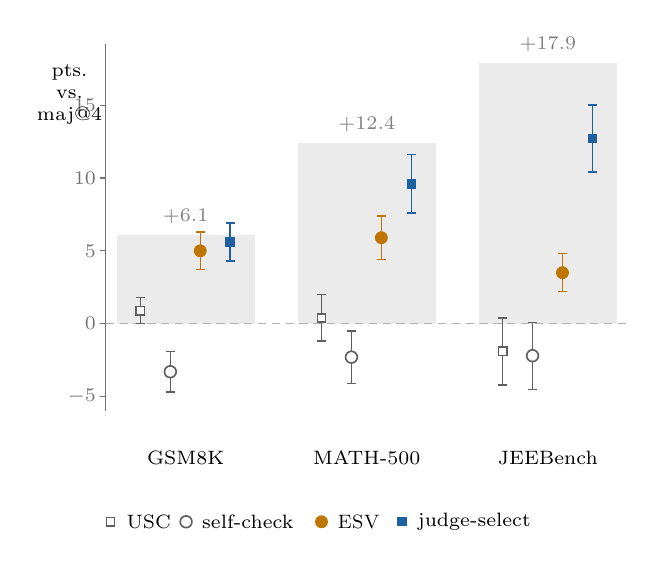
\begin{tikzpicture}[x=1cm, y=0.185cm, font=\footnotesize]
%% headroom: 0 up to the CoT pass@4 ceiling, the most any selector can gain
\fill[black!8] (0.70,0) rectangle (2.45,6.1);
\fill[black!8] (3.00,0) rectangle (4.75,12.4);
\fill[black!8] (5.30,0) rectangle (7.05,17.9);
\node[anchor=south, font=\scriptsize, black!50] at (1.575,6.2)  {$+6.1$};
\node[anchor=south, font=\scriptsize, black!50] at (3.875,12.5) {$+12.4$};
\node[anchor=south, font=\scriptsize, black!50] at (6.175,18.0) {$+17.9$};
%% axes
\draw[black!30, densely dashed] (0.56,0) -- (7.20,0);
\draw[black!55] (0.56,-6) -- (0.56,19.2);
\foreach \y in {-5,0,5,10,15}
  \draw[black!55] (0.49,\y) -- (0.56,\y) node[left=0pt, font=\scriptsize] {$\y$};
\node[anchor=south, font=\scriptsize, align=center] at (0.10,13.0) {pts.\\vs.\\maj@4};
%% benchmark labels
\node[font=\scriptsize] at (1.575,-9.2) {GSM8K};
\node[font=\scriptsize] at (3.875,-9.2) {MATH-500};
\node[font=\scriptsize] at (6.175,-9.2) {JEEBench};
%% ---- GSM8K
\ebar{1.00}{0.9}{0.9}{pgrey}   \mkopensq{(1.00,0.9)}{pgrey}
\ebar{1.38}{-3.3}{1.4}{pgrey}  \mkopenci{(1.38,-3.3)}{pgrey}
\ebar{1.76}{5.0}{1.3}{ccallb}  \mkfillci{(1.76,5.0)}{ccallb}
\ebar{2.14}{5.6}{1.3}{pblue}   \mkfillsq{(2.14,5.6)}{pblue}
%% ---- MATH-500
\ebar{3.30}{0.4}{1.6}{pgrey}   \mkopensq{(3.30,0.4)}{pgrey}
\ebar{3.68}{-2.3}{1.8}{pgrey}  \mkopenci{(3.68,-2.3)}{pgrey}
\ebar{4.06}{5.9}{1.5}{ccallb}  \mkfillci{(4.06,5.9)}{ccallb}
\ebar{4.44}{9.6}{2.0}{pblue}   \mkfillsq{(4.44,9.6)}{pblue}
%% ---- JEEBench
\ebar{5.60}{-1.9}{2.3}{pgrey}  \mkopensq{(5.60,-1.9)}{pgrey}
\ebar{5.98}{-2.2}{2.3}{pgrey}  \mkopenci{(5.98,-2.2)}{pgrey}
\ebar{6.36}{3.5}{1.3}{ccallb}  \mkfillci{(6.36,3.5)}{ccallb}
\ebar{6.74}{12.7}{2.3}{pblue}  \mkfillsq{(6.74,12.7)}{pblue}
%% legend
\mkopensq{(0.62,-13.6)}{pgrey} \node[anchor=west, font=\scriptsize] at (0.70,-13.6) {USC};
\mkopenci{(1.58,-13.6)}{pgrey} \node[anchor=west, font=\scriptsize] at (1.66,-13.6) {self-check};
\mkfillci{(3.30,-13.6)}{ccallb}\node[anchor=west, font=\scriptsize] at (3.38,-13.6) {\method{}};
\mkfillsq{(4.32,-13.6)}{pblue} \node[anchor=west, font=\scriptsize] at (4.40,-13.6) {judge-select};
\end{tikzpicture}
\caption{Accuracy change over CoT maj@4 with 95\% paired intervals. The grey
band runs to the pass@4 ceiling, the most any selector can gain. Self-check
(open circles) falls below zero everywhere and USC (open squares) straddles it.
Both gpt-oss-120b arms clear zero, but their gap widens with difficulty:
judge-select leads \method{} by 0.6, 3.7 and 9.2 points.}
\label{fig:gain}
\end{figure}

\subsection{Ablation Study}
\label{sec:ablation}

Table~\ref{tab:ablation} changes one component at a time. Swapping the checker for the solver reverses the sign of the gain everywhere, and dropping the structured form raises it everywhere. A cascade that keeps ESV and defers to judge-select only when ESV abstains recovers almost all of the difference but never beats judge-select alone (paired 0/2, 2/3, 2/2). Where ESV's rule commits to one candidate the two methods agree: they differ on 2 of 231 such GSM8K instances and on none of 187 on MATH-500. The structured form therefore decides only where ESV abstains. Nor is the rule the bottleneck: Section~\ref{sec:analysis} shows that the self-checker's verdict falls an order of magnitude short of the evidence any rule would need to overturn an untied vote, so no stage-3 rule reading those verdicts can recover the gap. The gate cannot change accuracy, since a unanimous instance offers nothing to select; without it ESV's GSM8K overhead would rise from 43.6\% to 168\% extra tokens.

\begin{table}[t]
\centering
\small
\setlength{\tabcolsep}{3pt}
\begin{tabular}{lrrr}
\toprule
$\Delta$ vs.\ maj@4 (points) & GSM8K & MATH & JEE \\
\midrule
ESV, gpt-oss-120b checker & +5.0 & +5.9 & +3.5 \\
\quad checker $\to$ the solver itself & $-3.3$ & $-2.3$ & $-2.2$ \\
\quad structured form $\to$ free-form & \textbf{+5.6} & \textbf{+9.6} & \textbf{+12.7} \\
\quad + free-form fallback on abstain & +5.5 & +9.5 & \textbf{+12.7} \\
\bottomrule
\end{tabular}
\caption{One change at a time from \method{} with the gpt-oss-120b checker;
free-form is judge-select. Each row changes exactly one component and leaves the
shared stage~0 samples, the candidate text and the scoring untouched. Removing
the gate leaves accuracy unchanged by construction, since a unanimous instance
offers nothing to select.}
\label{tab:ablation}
\end{table}

\subsection{Analysis}
\label{sec:analysis}

\paragraph{Why self-verification fails.}
On the GSM8K development split a candidate with one, two or three of four votes is correct 9.7, 51.1 and 77.8\% of the time. By Eq.~(2), overturning a 3--1 split then needs $\Lambda > 32.4$ and lifting a single-vote candidate in a 2--1--1 split needs $\Lambda > 9.7$; only ties need less. The self-checker's \textsc{sound} verdict carries $\Lambda = 1.6$ on GSM8K and 1.3 on MATH-500, and even \textsc{sound} on the challenger with \textsc{flawed} on the majority reaches only 2.3 and 1.7 if the verdicts are independent (Figure~\ref{fig:lr}). It cannot justify overturning any untied vote, whatever stage-3 rule reads it: the shortfall is in the evidence, not in the rule. gpt-oss-120b reaches 47.5, 11.8 and 48.9. The transcripts show the checker looking at the right evidence and misreading it. In 83\% of self-check calls on disagreeing breaking pairs (41 calls, development split) the checker's text engages the changed condition, yet it ratifies the solution that misuses it. In GSM8K pair 4 it quotes ``\$4 for each time she mows the lawn after the first 4 times'' word for word and then marks the trap's $4x$, which pays for every mowing, as \textsc{matches} (Appendix~\ref{app:transcripts}).

\begin{figure}[t]
\centering
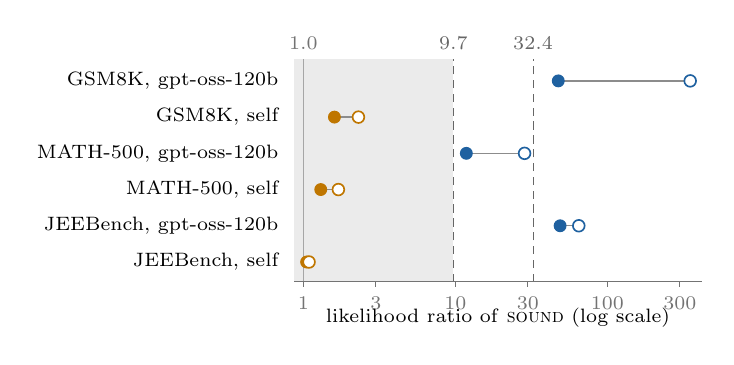
\begin{tikzpicture}[x=1.93cm, y=0.46cm, font=\footnotesize]
%% no untied vote can be overturned left of the 2--1--1 bar
\fill[black!8] (-0.06,0.45) rectangle (0.987,6.60);
%% Eq. (2) bars for the vote splits four samples allow
\draw[black!35] (0,0.45) -- (0,6.60)
  node[anchor=south, font=\scriptsize, black!55] {$1.0$};
\draw[black!60, densely dashed] (0.987,0.45) -- (0.987,6.60)
  node[anchor=south, font=\scriptsize] {$9.7$};
\draw[black!60, densely dashed] (1.511,0.45) -- (1.511,6.60)
  node[anchor=south, font=\scriptsize] {$32.4$};
%% x axis, decade ticks
\draw[black!55] (-0.06,0.45) -- (2.62,0.45);
\foreach \x/\lab in {0/1, 0.477/3, 1/10, 1.477/30, 2/100, 2.477/300}
  \draw[black!55] (\x,0.45) -- (\x,0.30) node[below=0pt, font=\scriptsize] {$\lab$};
\node[font=\scriptsize] at (1.28,-0.55) {likelihood ratio of \textsc{sound} (log scale)};
%% rows: filled = Lambda_S, open = Lambda_S+F, joined
\newcommand{\lrrow}[4]{%
  \node[anchor=east, font=\scriptsize] at (-0.10,#1) {#2};
  \draw[black!45, line width=.5pt] (#3,#1) -- (#4,#1);}
\lrrow{6}{GSM8K, gpt-oss-120b}{1.677}{2.545}
  \mkfillci{(1.677,6)}{pblue}  \mkopenci{(2.545,6)}{pblue}
\lrrow{5}{GSM8K, self}{0.204}{0.362}
  \mkfillci{(0.204,5)}{ccallb} \mkopenci{(0.362,5)}{ccallb}
\lrrow{4}{MATH-500, gpt-oss-120b}{1.072}{1.455}
  \mkfillci{(1.072,4)}{pblue}  \mkopenci{(1.455,4)}{pblue}
\lrrow{3}{MATH-500, self}{0.114}{0.230}
  \mkfillci{(0.114,3)}{ccallb} \mkopenci{(0.230,3)}{ccallb}
\lrrow{2}{JEEBench, gpt-oss-120b}{1.689}{1.812}
  \mkfillci{(1.689,2)}{pblue}  \mkopenci{(1.812,2)}{pblue}
\lrrow{1}{JEEBench, self}{0.021}{0.037}
  \mkfillci{(0.021,1)}{ccallb} \mkopenci{(0.037,1)}{ccallb}
\end{tikzpicture}
\caption{Likelihood ratio of a \textsc{sound} verdict (filled) against the
Eq.~(2) bars for the vote splits four samples allow (dashed): $32.4$ for 3--1,
$9.7$ for 2--1--1, and $1.0$ for a 2--2 tie. Five votes do not fit in four
samples, so no bar exists for a 2-vote challenger against a 3-vote majority.
Open circles add \textsc{flawed} on a competing candidate, assuming
independence. The self-checker (orange) never leaves the shaded region, where no
untied vote can be overturned; the independent checker (blue) clears the 2--1--1
bar everywhere.}
\label{fig:lr}
\end{figure}

\paragraph{Why the structured form loses.}
ESV abstains whenever no candidate is \textsc{sound} with zero \textsc{mismatch} and zero \textsc{violated} lines, and abstentions grow from 72 instances on GSM8K to 379 on MATH-500 and 612 on JEEBench. Of the fixable instances (majority wrong, some candidate right), ESV declines 8 of 71, 51 of 121 and 109 of 138 (Appendix~\ref{app:decisions}); on MATH-500 that is 50 abstentions plus one unreadable reply. The checker's false-positive rate stays at or below 5.2\%, but the share of correct candidates it passes falls from 86.7 to 60.8 to 25.0\%: one flagged line is enough to reject a candidate, and longer derivations plausibly offer more to flag. Judge-select also declines often, on 68.4\% of disagreeing JEEBench instances, but a correct candidate existed in only 6.1\% of those, and the candidates it does name are right 98.1\% of the time.

\paragraph{What the perturbations show.}
Breaking pairs cost the majority vote 11.5 points against originals on GSM8K and 13.7 on MATH-500, while preserving pairs score above originals on both (Appendix~\ref{app:arms}), so the difficulty comes from strategy misfit rather than novelty. On GSM8K, ESV gains most on breaking pairs (+8.4 points against +3.8 and +4.0). On originals, which the checker never solved during construction, it still gains +3.8 (23/1) on GSM8K and +6.7 (33/0) on MATH-500, so the construction overlap does not drive the result. The trap explains 18.5\% of wrong majority answers on GSM8K but only 5.6\% on MATH-500, so we confine the strategy-misfit reading to GSM8K. There, ESV's labels recover the trap's known cause above chance: 75.6\% of trap candidates are labeled \textsc{binding} errors against 55.7\% of other wrong candidates (OR 2.46, Fisher $p = 0.014$). The difference is not significant on MATH-500 ($p = 0.079$) and absent on JEEBench, and this interpretability on GSM8K is all the form adds.

\paragraph{Cost.}
ESV adds 43.6, 82.9 and 100.3\% tokens over maj@4, judge-select 20.7, 48.7 and 68.5\%, so ESV spends 2.4, 2.8 and 5.3 times as many tokens per net fix (Appendix~\ref{app:compute}). The gate's saving shrinks with difficulty: it skips 74.1\% of GSM8K instances but 10.1\% on JEEBench, where 46.2\% of the unanimous answers it waves through are wrong.
%% ======================================================================
\section{Discussion and Limitations}
%% ======================================================================
% Workshops value honesty here -- it also invites useful feedback.
Discuss when \method{} fails, assumptions it relies on, and open questions.

%% ======================================================================
\section{Conclusion and Future Work}
%% ======================================================================
Summarize the problem, approach, and key findings in 3--5 sentences, then
outline concrete next steps.

%% ======================================================================
%% OPTIONAL: ethics / broader impact (check if your workshop asks for it)
%% ======================================================================
% \section{Ethical Statement}
% Discuss potential misuse, data privacy, bias, or societal impact.

%% ======================================================================
%% ACKNOWLEDGMENTS -- camera-ready ONLY (reveals identity!)
%% ======================================================================
% \section{Acknowledgments}
% We thank \ldots{} This work was supported by \ldots

%% ======================================================================
%% REFERENCES
%% ======================================================================
\bibliography{aaai2027}   % your .bib file in the project root

%% ======================================================================
%% APPENDIX (optional; check your workshop's page-limit rules)
%% ======================================================================
\clearpage
\appendix
\renewcommand{\topfraction}{0.95}
\renewcommand{\bottomfraction}{0.9}
\renewcommand{\textfraction}{0.05}
\setcounter{topnumber}{4}
\setcounter{bottomnumber}{3}
\setcounter{totalnumber}{8}
\section{Appendix}

\subsection{Code and data}
\label{app:code}

The frozen perturbation sets, every raw model response, the decision-rule
implementation and the analysis scripts that regenerate each table and figure in
this paper are available at:

\begin{center}
\small\url{https://anonymous.4open.science/r/esv-anonymous}
\end{center}

\noindent
The release contains the three \texttt{frozen\_dataset.json} files with their
generation logs, the per-solver sample and verification records, and the
analyzer that emits the reports every number here is read from. No model call is
needed to reproduce a table: the stored responses are sufficient. The
de-anonymized repository link will replace the one above in the camera-ready
version.

\subsection{Datasets}
\label{app:data}

\begin{table}[!ht]
\centering
\small
\setlength{\tabcolsep}{3pt}
\begin{tabular}{@{}lrrr@{}}
\toprule
 & GSM8K & MATH-500 & JEEBench \\
\midrule
Usable source problems & 1{,}317 & 500 & 236 \\
Sampled (seed 2026) & 200 & 250 & 200 \\
Frozen pairs & 198 & 244 & 193 \\
\quad breaking/preserving & 99/99 & 123/121 & 97/96 \\
Acceptance, brk./pres. & 1.00/0.98 & 0.98/0.97 & 0.95/0.98 \\
Attempts (1/2/3+) & 182/16/0 & 216/23/5 & 155/25/13 \\
Solvers & 3 & 2 & 2 \\
Scored instances & 1{,}170 & 976 & 772 \\
Disagreeing & 25.9\% & 61.6\% & 89.9\% \\
Headroom (points) & 6.1 & 12.4 & 17.9 \\
\bottomrule
\end{tabular}
\caption{The frozen perturbation sets. Instances count $P$ and $P'$ once per
solver. Acceptance is the share of attempted perturbations the two verifiers
accepted, per mode; attempts counts how many generations a frozen pair needed.
GSM8K drops two source problems with negative answers and excludes six
originals with disputed gold answers, leaving 390 instances per solver.}
\label{tab:datasets}
\end{table}

Table~\ref{tab:datasets} summarises the three frozen sets.
GSM8K answers are all integers. MATH-500 keeps 145 integer, 88 expression and 11 numeric answers, and its 244 pairs span levels 1--5 (20/43/58/61/62) and all seven subjects (Algebra 59, Intermediate Algebra 47, Prealgebra 44, Precalculus 30, Number Theory 27, Geometry 21, Counting and Probability 16). JEEBench mathematics answers are multiple-correct (68), numeric (55), single-correct (41) and integer (29). Expression answers are compared by a normalizer that tries canonical and case-insensitive string equality, element-wise comparison of tuples, intervals, sets and vectors with matching delimiters, exact numeric equality, and finally a symbolic check that is abandoned unless the \LaTeX{} conversion is complete; a decimal approximation of an exact value is never accepted. A hand audit of 19 GSM8K pairs found every accepted answer correct. The six excluded GSM8K originals are pairs 40, 82, 95, 105, 111 and 189; their perturbed siblings keep their verified answers. On GSM8K the held-out split (pairs 60--197) gives maj@4 88.8\%, USC 89.7\%, self-check ESV 85.1\%, ESV with gpt-oss-120b 94.1\% and pass@4 95.1\%; the development split gives 87.7, 88.5, 85.2, 92.2 and 93.3\%. The judge-select control was designed and run after the held-out evaluation and was not part of the pre-registered criterion.

\subsection{Exact tests and confidence intervals}
\label{app:pvalues}

Table~\ref{tab:pvalues} gives, for every method, the accuracy change against CoT maj@4, a 95\% confidence interval for a paired difference in proportions, and the exact two-sided McNemar $p$-value on the discordant instances. Table~\ref{tab:h2h} gives the head-to-head comparisons quoted in the text.

\begin{table*}[t]
\centering
\small
\setlength{\tabcolsep}{3pt}
\begin{tabular}{lrrrrrr}
\toprule
 & \multicolumn{2}{c}{GSM8K} & \multicolumn{2}{c}{MATH-500} & \multicolumn{2}{c}{JEEBench} \\
\cmidrule(lr){2-3}\cmidrule(lr){4-5}\cmidrule(lr){6-7}
Method & $\Delta \pm$ CI & $p$ & $\Delta \pm$ CI & $p$ & $\Delta \pm$ CI & $p$ \\
\midrule
Direct QA & $-76.3 \pm 2.5$ & 2e-256 & $-45.7 \pm 3.4$ & 6e-110 & $-12.0 \pm 3.6$ & 8e-11 \\
USC & $+0.9 \pm 0.9$ & 0.087 & $+0.4 \pm 1.6$ & 0.71 & $-1.9 \pm 2.3$ & 0.11 \\
ESV, self & $-3.3 \pm 1.4$ & 7e-06 & $-2.3 \pm 1.8$ & 0.017 & $-2.2 \pm 2.3$ & 0.078 \\
ESV, 120b & $+5.0 \pm 1.3$ & 4e-16 & $+5.9 \pm 1.5$ & 1e-16 & $+3.5 \pm 1.3$ & 1e-07 \\
Judge-select & $+5.6 \pm 1.3$ & 5e-19 & $+9.6 \pm 2.0$ & 1e-23 & $+12.7 \pm 2.3$ & 6e-30 \\
pass@4 & $+6.1 \pm 1.4$ & 8e-22 & $+12.4 \pm 2.1$ & 8e-37 & $+17.9 \pm 2.7$ & 6e-42 \\
\bottomrule
\end{tabular}
\caption{Change in accuracy over CoT maj@4 (points) with a 95\% paired Wald interval, and exact two-sided McNemar $p$.}
\label{tab:pvalues}
\end{table*}

\begin{table}[!ht]
\centering
\small
\setlength{\tabcolsep}{4pt}
\begin{tabular}{@{}lccc@{}}
\toprule
Comparison & GSM8K & MATH-500 & JEEBench \\
\midrule
\method{} vs.\ USC   & 53 / 4 & 71 / 17 & 69 / 27 \\
                     & 6e-12 & 5e-09 & 2e-05 \\
\method{} vs.\ Judge & 0 / 7 & 4 / 40 & 2 / 73 \\
                     & 0.016 & 2e-08 & 2e-19 \\
Cascade vs.\ Judge   & 0 / 2 & 2 / 3 & 2 / 2 \\
                     & 0.50 & 1.00 & 1.00 \\
Self-check vs.\ USC  & 17 / 66 & 35 / 61 & 45 / 47 \\
                     & 6e-08 & 0.010 & 0.92 \\
\bottomrule
\end{tabular}
\caption{Paired head-to-head comparisons on the same instances, with \method{}
using the gpt-oss-120b checker unless stated and Judge the judge-select control.
The first line of each block gives wins / losses for the left-hand method, the
second the exact two-sided McNemar $p$. The cascade runs \method{} and falls
back to judge-select when no candidate passes the strict rule.}
\label{tab:h2h}
\end{table}

\subsection{Decisions, selection quality and verifier rates}
\label{app:decisions}

Table~\ref{tab:decisions} breaks ESV's outcomes down by what the decision rule did. The last column counts instances where the majority was wrong, a candidate was right, and the rule abstained; these are the gains a looser rule could still reach. Table~\ref{tab:selection} restricts accuracy to disagreeing instances, the only ones a selector can change, and Table~\ref{tab:detector} gives the per-candidate verifier rates behind Figure~\ref{fig:lr}.

\begin{table}[!ht]
\centering
\small
\setlength{\tabcolsep}{3pt}
\begin{tabular}{@{}lrrrrr@{}}
\toprule
Rule outcome & $n$ & maj@4 & \method{} & $F$ / $B$ & Decl. \\
\midrule
\multicolumn{6}{@{}l}{\textit{GSM8K} (1{,}170)} \\
\quad unanimous      & 867 & 98.0 & 98.0 & --     & -- \\
\quad one sound      & 231 & 70.6 & 96.1 & 61 / 2 & -- \\
\quad none (abstain) &  72 & 30.6 & 30.6 & --     & 8 \\
\midrule
\multicolumn{6}{@{}l}{\textit{MATH-500} (976)} \\
\quad unanimous      & 375 & 96.0 & 96.0 & --     & -- \\
\quad one sound      & 187 & 59.4 & 89.3 & 57 / 1 & -- \\
\quad several sound  &  34 & 38.2 & 44.1 & 2 / 0  & -- \\
\quad none (abstain) & 379 & 17.4 & 17.4 & --     & 50 \\
\quad unreadable     &   1 &  0.0 &  0.0 & --     & 1 \\
\midrule
\multicolumn{6}{@{}l}{\textit{JEEBench} (772)} \\
\quad unanimous      &  78 & 53.8 & 53.8 & --     & -- \\
\quad one sound      &  75 & 56.0 & 92.0 & 28 / 1 & -- \\
\quad several sound  &   2 &  0.0 &  0.0 & 0 / 0  & -- \\
\quad none (abstain) & 612 & 16.5 & 16.5 & --     & 109 \\
\quad unreadable     &   5 &  0.0 &  0.0 & --     & -- \\
\bottomrule
\end{tabular}
\caption{\method{} (gpt-oss-120b) by decision-rule outcome; accuracies in \%.
``one sound'' is the branch that commits to a candidate, ``Decl.'' counts
fixable instances (majority wrong, a candidate right) on which the rule
abstained. GSM8K has no \emph{several sound} or \emph{unreadable} instances, so
those rows are absent rather than zero. The rows sum to the scored instances of
each benchmark.}
\label{tab:decisions}
\end{table}

\begin{table}[!ht]
\centering
\small
\setlength{\tabcolsep}{4pt}
\begin{tabular}{@{}lrrr@{}}
\toprule
Selector & GSM8K & MATH & JEE \\
$n$ disagreeing & 303 & 601 & 694 \\
\midrule
Random candidate & 37.0 & 20.0 & 15.6 \\
Majority vote & 61.1 & 31.6 & 20.6 \\
USC & 64.4 & 32.3 & 18.4 \\
\method{}, self-check & 48.2 & 28.0 & 18.2 \\
\method{}, gpt-oss-120b & 80.5 & 41.3 & 24.5 \\
Judge-select & \textbf{82.8} & \textbf{47.3} & \textbf{34.7} \\
Oracle (pass@4) & 84.5 & 51.7 & 40.5 \\
\bottomrule
\end{tabular}
\caption{Selection quality: accuracy (\%) on instances whose four samples disagree. The random-candidate row is the expected accuracy of drawing one candidate uniformly, averaged over instances.}
\label{tab:selection}
\end{table}

\begin{table}[!ht]
\centering
\small
\setlength{\tabcolsep}{3pt}
\begin{tabular}{@{}llrrrrr@{}}
\toprule
 & Check & TPR & FPR & Prec. & $\Lambda_{\textsc{s}}$ & $\Lambda_{\textsc{s}+\textsc{f}}$ \\
\midrule
GSM8K & self & 57.0 & 36.5 & 44.8 & 1.6 & 2.3 \\
      & 120b & 86.7 & 1.8 & 96.1 & 47.5 & 351 \\
MATH  & self & 56.3 & 43.3 & 20.7 & 1.3 & 1.7 \\
      & 120b & 60.8 & 5.2 & 70.3 & 11.8 & 28.5 \\
JEE   & self & 44.6 & 42.5 & 14.3 & 1.1 & 1.1 \\
      & 120b & 25.0 & 0.5 & 88.6 & 48.9 & 64.9 \\
\bottomrule
\end{tabular}
\caption{Per-candidate verifier rates; ``120b'' is gpt-oss-120b. TPR and FPR
are the shares of correct and of wrong candidates judged strictly
\textsc{sound}, Prec.\ the precision of that verdict.
$\Lambda_{\textsc{s}}$ is its likelihood ratio and
$\Lambda_{\textsc{s}+\textsc{f}}$ multiplies in \textsc{flawed} on a competing
candidate, assuming independence. Candidates: 256/493, 311/1{,}552 and
280/1{,}760 correct/wrong.}
\label{tab:detector}
\end{table}

When judge-select names a candidate, that candidate is correct 96.5\% (GSM8K), 89.6\% (MATH-500) and 98.1\% (JEEBench) of the time; it answers NONE on 15.2\%, 49.8\% and 68.4\% of disagreeing instances.

\subsection{Perturbation arms and answer formats}
\label{app:arms}

Table~\ref{tab:arms} splits every instance by which arm of the pair it came
from: the untouched original $P$, a strategy-breaking $P'$, or a
strategy-preserving $P'$. The breaking arm is the one \method{} was designed
for, so the fixes-and-breaks column is read per arm.

\begin{table}[t]
\centering
\small
\setlength{\tabcolsep}{3.5pt}
\begin{tabular}{@{}llrrrr@{}}
\toprule
 & Arm & $n$ & maj@4 & \method{} & $F$ / $B$ \\
\midrule
GSM8K & originals & 576 & 90.6 & 94.4 & 23 / 1 \\
      & breaking $P'$ & 297 & 79.1 & 87.5 & 25 / 0 \\
      & preserv.\ $P'$ & 297 & 93.6 & 97.6 & 13 / 1 \\
\midrule
MATH  & originals & 488 & 57.6 & 64.3 & 33 / 0 \\
      & breaking $P'$ & 246 & 43.9 & 50.0 & 16 / 1 \\
      & preserv.\ $P'$ & 242 & 66.5 & 70.7 & 10 / 0 \\
\midrule
JEE   & originals & 386 & 23.6 & 26.4 & 11 / 0 \\
      & breaking $P'$ & 194 & 24.7 & 27.8 & 7 / 1 \\
      & preserv.\ $P'$ & 192 & 24.0 & 29.2 & 10 / 0 \\
\bottomrule
\end{tabular}
\caption{Accuracy (\%) by perturbation arm, ESV with gpt-oss-120b. USC on GSM8K scores 91.5, 79.8 and 94.6 on the three arms. Only on GSM8K and MATH-500 does the breaking arm sit below the originals; on JEEBench the three arms are within 1.1 points of each other, which is why we confine the strategy-misfit reading to the first two.}
\label{tab:arms}
\end{table}

On GSM8K the trap answer accounts for 25 of the 135 wrong majority answers (18.5\%) and appears in 90 of the 1{,}188 samples drawn on breaking pairs (7.6\%); 54 of the wrong answers (40.0\%) are on unperturbed originals. On MATH-500 the trap accounts for 24 of 426 wrong answers (5.6\%).

MATH-500 answers come in three formats. ESV's gain is similar across them: expression answers (352 instances) rise from 40.6 to 46.0\% (20/1), integers (580) from 65.5 to 71.9\% (37/0) and numeric answers (44) from 61.4 to 65.9\% (2/0). The expression scorer is therefore not what separates the methods.

\subsection{Error attribution}
\label{app:attribution}

On a breaking pair, a candidate equal to the trap applies the original strategy as if the changed condition still held, so its cause is known. Table~\ref{tab:attribution} compares ESV's failure-type labels on these candidates with its labels on other wrong candidates. The labels are informative but not specific: 37--61\% of all wrong candidates are labeled \textsc{binding}.

\begin{table*}[!ht]
\centering
\small
\setlength{\tabcolsep}{3pt}
\begin{tabular}{llrrrrr}
\toprule
 & Candidate group & $n$ & \textsc{bind.} & \textsc{meth.} & \textsc{comp.} & \textsc{sound} \\
\midrule
GSM8K & trap (known cause) & 45 & 75.6 & 17.8 & 6.7 & 0.0 \\
 & other wrong, breaking & 193 & 60.6 & 15.0 & 24.4 & 0.0 \\
 & wrong, orig.\ or pres. & 255 & 55.7 & 9.8 & 31.0 & 3.5 \\
 & correct & 256 & 9.8 & 1.6 & 2.0 & 86.7 \\
\midrule
MATH-500 & trap & 43 & 51.2 & 27.9 & 20.9 & 0.0 \\
 & wrong, orig.\ or pres. & 1{,}062 & 37.5 & 24.9 & 31.2 & 6.2 \\
\midrule
JEEBench & trap & 57 & 42.1 & 31.6 & 21.1 & 3.5 \\
 & wrong, orig.\ or pres. & 1{,}320 & 46.9 & 29.5 & 22.7 & 0.3 \\
\bottomrule
\end{tabular}
\caption{ESV's failure-type labels (\% of candidates, gpt-oss-120b checker) by ground-truth group. A trap candidate is a \textsc{binding} error by construction. Trap against other wrong candidates on originals and preserving pairs, \textsc{binding} rate: GSM8K OR 2.46 ($p$=0.014), MATH-500 OR 1.75 ($p$=0.079), JEEBench OR 0.82 ($p$=0.501), Fisher exact test.}
\label{tab:attribution}
\end{table*}

\subsection{Compute}
\label{app:compute}

Table~\ref{tab:compute} gives the cost of every method per instance and
Figure~\ref{fig:cost} plots what that cost buys. Both are read off the
\texttt{usage} and latency fields stored on each call, so they reproduce offline
from the records.

\begin{table*}[!ht]
\centering
\small
\setlength{\tabcolsep}{3pt}
\begin{tabular}{llrrrr}
\toprule
 & Method & Tokens & vs.\ maj@4 & Crit.\ path (s) & Tok./net fix \\
\midrule
GSM8K & CoT maj@4 & 2{,}379 & -- & 6.5 & -- \\
 & USC & 2{,}799 & +17.6\% & 6.7 & 49.1k \\
 & ESV, self & 3{,}158 & +32.7\% & 10.8 & no gain \\
 & Judge-select & 2{,}871 & +20.7\% & 10.0 & \textbf{8.7k} \\
 & ESV, 120b & 3{,}417 & +43.6\% & 13.7 & 20.6k \\
\midrule
MATH-500 & CoT maj@4 & 4{,}592 & -- & 31.8 & -- \\
 & USC & 6{,}159 & +34.1\% & 32.6 & 382k \\
 & ESV, self & 7{,}433 & +61.9\% & 55.6 & no gain \\
 & Judge-select & 6{,}826 & +48.7\% & 44.7 & \textbf{23.2k} \\
 & ESV, 120b & 8{,}399 & +82.9\% & 72.9 & 64.1k \\
\midrule
JEEBench & CoT maj@4 & 7{,}548 & -- & 31.4 & -- \\
 & USC & 10{,}910 & +44.5\% & 32.2 & no gain \\
 & ESV, self & 12{,}411 & +64.4\% & 55.6 & no gain \\
 & Judge-select & 12{,}718 & +68.5\% & 73.0 & \textbf{40.7k} \\
 & ESV, 120b & 15{,}116 & +100.3\% & 92.0 & 216k \\
\bottomrule
\end{tabular}
\caption{Cost per instance. Tokens are prompt plus completion summed over solver and checker; the critical path is the latency a user waits, since the four samples run concurrently. Tokens per net fix is extra tokens times $N$ divided by $F-B$. Solver and checker tokens are counted at equal weight.}
\label{tab:compute}
\end{table*}

\begin{figure}[t]
\centering
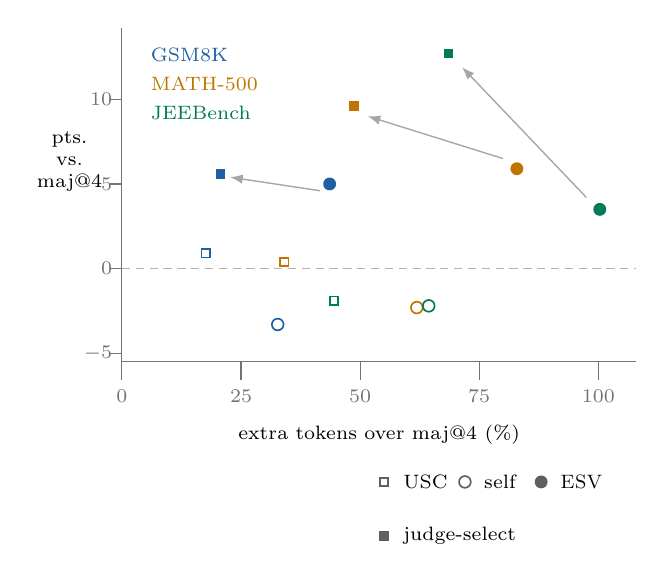
\begin{tikzpicture}[x=0.0605cm, y=0.215cm, font=\footnotesize]
%% axes: x = extra tokens as a share of the maj@4 baseline, y = points over maj@4
\draw[black!30, densely dashed] (0,0) -- (108,0);
\draw[black!55] (0,-5.5) -- (0,14.2);
\draw[black!55] (0,-5.5) -- (108,-5.5);
\foreach \y in {-5,0,5,10}
  \draw[black!55] (-2.5,\y) -- (0,\y) node[left=0pt, font=\scriptsize] {$\y$};
\foreach \x in {0,25,50,75,100}
  \draw[black!55] (\x,-5.5) -- (\x,-6.6) node[below=0pt, font=\scriptsize] {$\x$};
\node[font=\scriptsize] at (54,-9.8) {extra tokens over maj@4 (\%)};
\node[anchor=south, font=\scriptsize, align=center] at (-11,4.0) {pts.\\vs.\\maj@4};
%% the move from ESV to judge-select: up and to the left on every benchmark
\draw[-{Latex[length=1.6mm]},black!35,line width=.5pt] (41.6,4.6) -- (22.7,5.4);
\draw[-{Latex[length=1.6mm]},black!35,line width=.5pt] (80.0,6.5) -- (51.6,9.0);
\draw[-{Latex[length=1.6mm]},black!35,line width=.5pt] (97.5,4.2) -- (71.4,11.9);
%% GSM8K (blue)
\mkopensq{(17.6,0.9)}{pblue}  \mkopenci{(32.7,-3.3)}{pblue}
\mkfillci{(43.6,5.0)}{pblue}  \mkfillsq{(20.7,5.6)}{pblue}
%% MATH-500 (orange)
\mkopensq{(34.1,0.4)}{ccallb} \mkopenci{(61.9,-2.3)}{ccallb}
\mkfillci{(82.9,5.9)}{ccallb} \mkfillsq{(48.7,9.6)}{ccallb}
%% JEEBench (green)
\mkopensq{(44.5,-1.9)}{pgreen}\mkopenci{(64.4,-2.2)}{pgreen}
\mkfillci{(100.3,3.5)}{pgreen}\mkfillsq{(68.5,12.7)}{pgreen}
%% legends
\node[anchor=west, font=\scriptsize, pblue]  at (4,12.6) {GSM8K};
\node[anchor=west, font=\scriptsize, ccallb] at (4,10.9) {MATH-500};
\node[anchor=west, font=\scriptsize, pgreen] at (4,9.2)  {JEEBench};
\mkopensq{(55,-12.6)}{pgrey} \node[anchor=west, font=\scriptsize] at (57,-12.6) {USC};
\mkopenci{(72,-12.6)}{pgrey} \node[anchor=west, font=\scriptsize] at (74,-12.6) {self};
\mkfillci{(88,-12.6)}{pgrey} \node[anchor=west, font=\scriptsize] at (90,-12.6) {\method{}};
\mkfillsq{(55,-15.8)}{pgrey} \node[anchor=west, font=\scriptsize] at (57,-15.8) {judge-select};
\end{tikzpicture}
\caption{Accuracy gain against extra tokens, both over CoT maj@4, with color
for the benchmark and shape for the method. Judge-select sits up and to the left
of \method{} on all three (arrows): cheaper and more accurate. Every method
issues the same single extra call, so the spread along the $x$ axis is reply
length alone --- \method{}'s per-candidate form costs 1.5 to 2.1 times the
checker tokens free-form adjudication does.}
\label{fig:cost}
\end{figure}

The gate fires on 25.9\%, 61.6\% and 89.9\% of instances. A verification call on a GSM8K instance that reaches it costs 4{,}008 tokens and 27.8 seconds; amortized over all instances it costs 1{,}038 tokens and 7.2 seconds. The gate also directs spending where the errors are: it fires on 45.1\% of breaking $P'$ against 17.5\% of preserving $P'$. Counting checker tokens at $k$ times the price of solver tokens, ESV costs less per net fix than USC for $k < 2.4$ on GSM8K and $k < 6.0$ on MATH-500. USC's total gain is capped at 10 net fixes on GSM8K against ESV's 59, so additional USC spending cannot reach ESV's accuracy.

\subsection{Large solvers}
\label{app:large}

With Qwen2.5-72B-Instruct, Mistral-Small-3.2-24B and Llama-3.3-70B as solvers on GSM8K (1{,}170 instances), CoT maj@4 reaches 96.9\% (96.9, 96.7 and 97.2\% per solver) and pass@4 99.0\%. Only 88 instances disagree, 24 of them fixable, and one of the 1{,}082 unanimous instances is wrong. With 2.1 points of headroom there is little for any selector to recover, so we report this arm as the reason the small solvers are the test and did not run verification on it.

\subsection{Verification transcripts}
\label{app:transcripts}

Both examples come from the self-check arm on the GSM8K development split.

\noindent\fbox{\parbox{0.95\columnwidth}{\small
\textbf{Pair 4 (breaking).} The perturbed problem pays Sara nothing for her first four mowings. The checker quotes the clause ``\$4 for each time she mows the lawn after the first 4 times'' word for word, then marks the trap solution's binding $4x$, which pays for every mowing, as \textsc{matches} and returns \textsc{sound}.}}

\vspace{4pt}
\noindent\fbox{\parbox{0.95\columnwidth}{\small
\textbf{Pair 36 (breaking).} The first leg of a relay is shortened to 380\,m while the nominal times stay unchanged. The checker writes that the first runner runs 380\,m in 60\,s and marks the condition \textsc{holds}, calls the trap solution's per-meter rescaling correct, and argues for the trap in its divergence analysis.}}

\subsection{Prompt note}

During development the CoT and Direct QA prompts told every model to answer multiple-choice questions with an option letter, and Gemma-3-4B returned a bare letter on 138 of 168 GSM8K samples. The instruction now depends on the answer format (integer, numeric or expression), with the multiple-choice wording unchanged for JEEBench. Every run reported in this paper carries the same prompt build, \texttt{jee\_methods\_v1\_2026-11-01}, and no bare option letter survives in any of the 17{,}312 stored GSM8K and MATH-500 samples.
\end{document}
